
\section{Análisis de Requisitos}


En esta aplicación móvil objetivo de este proyecto, se establecieron una serie de requisitos que debería cumplir la aplicación. Estos requisitos fueron obtenidos al  hacer una entrevista con los directores del proyecto.\\

El registro del usuario sería el primero para poder darle acceso y comenzar a usarla, ya que sin el no tiene acceso a ninguna funcionalidad de la aplicación.

La creación de puntos de interés marcados en un mapa con nombre, descripción y un punto en el mapa con o sin señal GPS clasificados en tipo, caza o pesca. \\

Creación y almacenamiento de las rutas seguidas por un usuario en sus caminatas por cualquier tipo de terrero.\\

El usuario también podrá crear grupos con los usuarios que le parezca oportuno y los integrantes del mismo poder añadir a otros. E resultado de esta funcionalidad es la que permitirá posteriormente crear rutas conjuntas ya para crear una ruta conjunta primero se elige el grupo del que se hará el seguimiento. Una vez elegido se enviarán las invitaciones para participar en él a cada integrante del grupo. Estas invitaciones en el caso de ser aceptadas permitirán al usuario navegar por un mapa y periódicamente se irán realizando actualizaciones de las posiciones del resto de integrantes. Finalmente se podrán ver las rutas conjuntas igual que las individuales.
\subsection{Actores}

Los únicos actores que se presentan en la  aplicación son los siguientes:
\begin{itemize}
\item \textbf{Usuario no  autenticado}. Usuario que no está autenticado en la aplicación y que solo
se le permite registrarse en el  sistema o iniciar sesión si la ya se registro en otro momento.
\item \textbf{Usuario  autenticado}. Usuario autenticado que puede acceder a todas as funcionalidades
del sistema.
\end{itemize}


\section{Historias de usuario}
Historias de Usuario son los requisitos vistos desde el punto de vista del usuario, es decir, acciones que el usuario llevará a cabo durante el uso del la aplicación. Son la unidad básica en cada Sprint y se caracteriza por ser:
\begin{itemize}
\item Independientes
 \item Negociables
  \item Estimables
  \item Pequeñas
   \item Tangibles
    
\end{itemize}

Las historias en este proyecto serán las siguientes:


\begin{itemize}
 \item Gestión de puntos de interés (PDI)
\item Iniciar sesión  
  \item Gestión de grupos
  \item Iniciar una ruta individual
   \item Iniciar la ruta compartida
    
\end{itemize}
 Estas historias anteriormente citadas serán divididas en cada Sprint en pequeñas tareas mas fáciles de manejar. Una tarea es la acción que debe implementar el desarrollador para que se pueda ejecutar parte de la historia, esta está en un lenguaje técnico. Estas tareas pasar a ser en la mayoría de los casos a ser lo denominados casos de uso que comentaremos posteriormente.

\subsection{Casos de uso}
A continuación, en esta sección, se exponen los requisitos funcionales que surgen de los requisitos generales planteados en el punto anterior.
\subsubsection{• Usuario no autenticado}
\begin{itemize}
\item\textbf{ \textit{R1}  Registrarse en la aplicación.}
 El usuario podrá darse de alta en el sistema
introduciendo sus datos en el formulario que se le indican. Una vez registrado se iniciará sesión
automáticamente con el nuevo perfil.

\item \textbf{\textit{R2} Iniciar sesión en la aplicación. }
El usuario ya registrado podrá, con
sus credenciales, autenticarse en el  sistema. Se pedirá el nombre del usuario y su contraseña. Se guardará el estado en el terminal hasta que el usuario decida desconectarse.
\end{itemize} 
\begin{figure}[H]
		\centering
		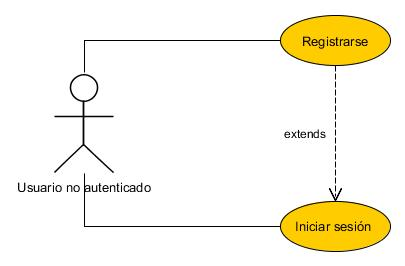
\includegraphics[width=0.75\textwidth] {usuario-no-autenticado.jpg}
		\caption{Casos de uso del actor Usuario No Autenticado }
	\end{figure}
	
	
	
\subsubsection{• Usuario  autenticado}

Para el caso de que el usuario ya esté autenticado dividiremos en 3 grupos los casos de usos:
\begin{itemize}
\item \textbf{Gestión de puntos de interés}\\
Aquí se describirán los casos de uso relacionados con la gestión  de la información del los puntos de interés.
\begin{itemize}
\item\textbf{\textit{ R-PDI-1 Guardar Punto De Interés caza}}, el usuario podrá guardar un punto concreto, de caza, asociado a un par de coordenadas pudiendo añadirle un nombre y una descripción.
\item\textit{ \textbf{R-PDI-2 Guardar Punto De Interés pesca}}, el caso de uso es similar al de anterior pero este es para el tipo de pesca.
\item \textbf{\textit{R-PDI-3 Eliminar PDI}}, el usuario podrá seleccionar un punto o una lista de puntos para ser borrados.
\item \textbf{\textit{R-PDI-4 Buscar los PDI}}, permite ver todos los puntos de interés de cada tipo en un mapa y pudiendo clicar en ellos para conocer su nombre y descripción.
\end{itemize} 

\begin{figure}[H]
		\centering
		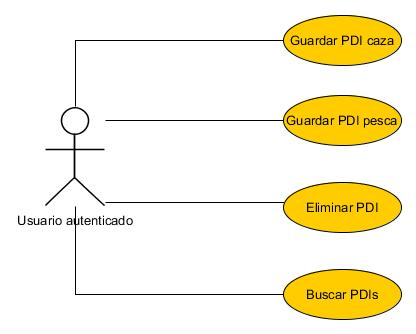
\includegraphics[width=0.75\textwidth] {PDI.jpg}
		\caption{Casos de uso de gestión de puntos de interés }
	\end{figure}
	
	
	
\item \textbf{Gestión de grupos}
\begin{itemize}
\item\textbf{ \textit{R-G-1 Crear grupo}}, el usuario crea un grupo con nombre único.
\item\textbf{\textit{ R-G-2 Añadir integrantes}}, el usuario busca en la base de datos los usuarios que quiere integrar en el grupo previamente seleccionado.
\item \textbf{\textit{R-G-3 Eliminar integrantes}}, el usuario puede eliminar los integrantes que vea pertinentes.
\item \textbf{\textit{R-G-4 Ver grupos}}, el sistema listar los grupos en los que el usuario está registrado.
\item \textbf{\textit{R-G-5 Ver integrantes grupo}}, el sistema permitirá ver los integrantes del grupo que el usuario indique, previo listado del caso de uso R-G-4. 

\end{itemize} 

\begin{figure}[H]
		\centering
		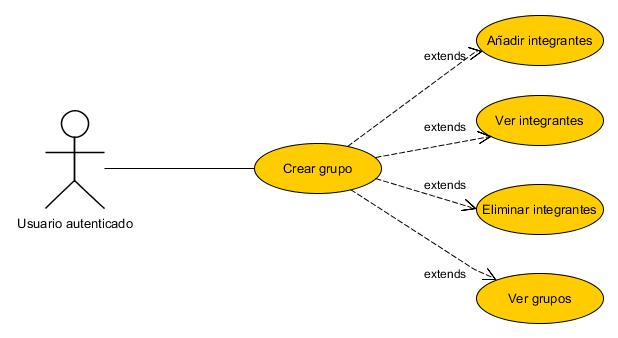
\includegraphics[width=0.75\textwidth] {grupo.jpg}
		\caption{Casos de uso de gestión de grupos de usuarios }
	\end{figure}
	
	
	
\item \textbf{Gestión de rutas}, el usuario iniciará una navegación privada siendo guardada la ruta seguida.
\begin{itemize}
\item \textbf{\textit{R-R-1 Crear ruta privada}}, el usuario registra la ruta con un nombre.
\begin{itemize}
\item \textbf{\textit{R-R-1.1}} Iniciar ruta, el sistema comienza a guardar las coordenadas por la que el usuario esta navegando y dibujando la ruta en el mapa. Las coordenadas se irán guardando periódicamente, no solo al finalizar la ruta y visualizarla.
\item\textbf{ \textit{R-R-1.2}} Parar ruta, permite parar la navegación, tanto de guardar las coordenadas como de pintar la ruta seguida.
\item \textbf{\textit{R-R-1.3}} Guardar ruta, el sistema guarda los últimos puntos que quedaban sin actualizar y ejecuta el caso de uso ver ruta en el mapa(R-R-4).
\end{itemize}

\item \textbf{\textit{R-R-2 Crear ruta compartida}}, este caso de uso permite guardar la ruta seguida por el usuario y al mismo tiempo ver la posición del resto de integrantes de un grupo, anteriormente seleccionado, en tiempo real. Este caso de uso también enviaría a los integrantes del grupo una invitación a dicha ruta.
\begin{itemize}
\item \textbf{\textit{R-R-2.1 Iniciar ruta}}, se comienza a guardar y dibujar la ruta en el mapa. Por otra parte se comienza el seguimiento del resto de usuario que estén también navegando. Como también una actualización parcial de la ruta seguida en el servidor.
\item \textbf{\textit{R-R-2.2 Parar ruta}}, se para la navegación y se deja de actualizar la posición al resto de usuario de la ruta compartida.
\item \textbf{\textit{R-R-2.3 Finalizar ruta}}, se guardan los puntos que faltan de enviar al servidor y se deja de enviar datos al resto de integrantes.
\end{itemize}
\item \textbf{\textit{R-R-3 Listar rutas} }, permite al usuario ver todas las rutas realizadas tanto de manera privada como de manera compartida.
\item \textbf{\textit{R-R-4 Ver ruta en mapa}}, el sistema dibuja en un mapa la ruta seguida y previamente seleccionada.
\item \textbf{\textit{R-R-5 Eliminar ruta}}, permite al usuario borrar de la aplicación la ruta indicada.

\end{itemize} 
\end{itemize}
\begin{figure}[H]
		\centering
		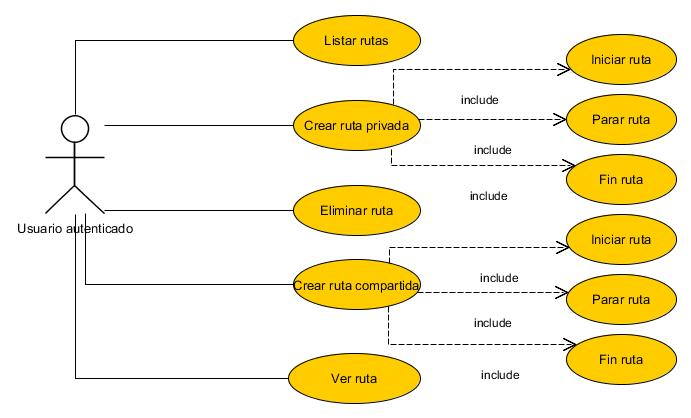
\includegraphics[width=0.75\textwidth] {rutas.jpg}
		\caption{Casos de uso de gestión de rutas }
	\end{figure}


\section{Análisis de riesgos}
\subsection{Riesgos identificados}
\begin{figure}[H]
		\centering
		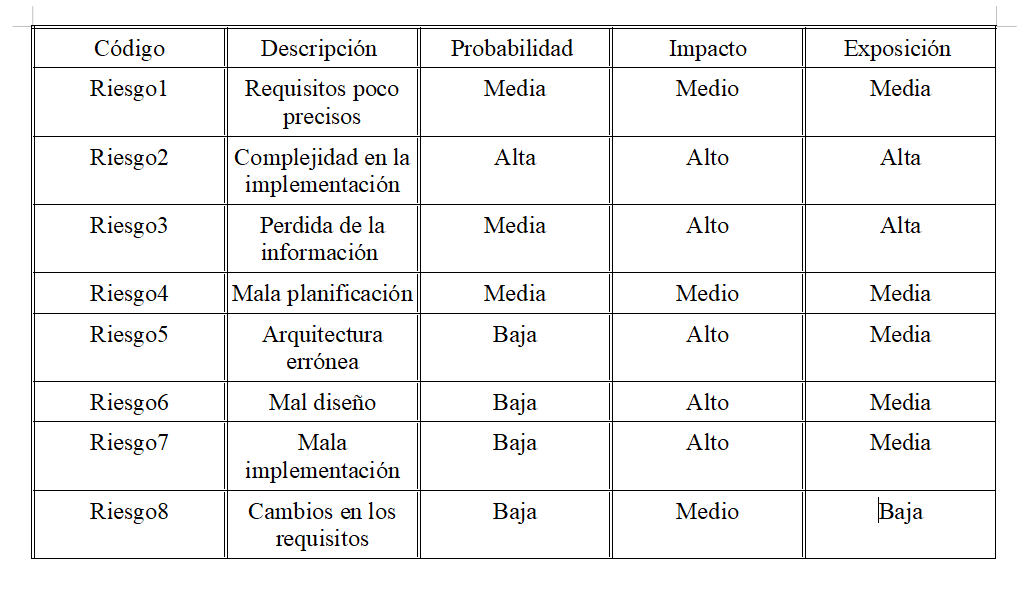
\includegraphics[width=0.75\textwidth] {riesgos.png}
		\caption{Identificación y clasificación de riesgos del proyecto }
	\end{figure}
	
	
Una vez identificados y clasificados los riesgos debemos realizar dos acciones diferentes dependiendo del riesgo que conlleven:
\subsection{Planes de contingencia} 

Los riesgos que tengan una alta exposición pueden hacer peligrar el futuro del proyecto por ello,  debemos analizarlos en fases tempranas, antes
de comenzar el diseño o la implementación, y que así   vigilarlos. En el caso de este proyecto la manera de solventarlos fue diferente.  A continuación de comentan.

 

\begin{itemize}
\item \textbf{Riesgo1} \textbf{- Curva aprendizaje Android}. Este riesgo era algo que se conocía antes de comenzar ya con el proyecto y por ello era algo que se tenía  muy en cuenta. Para atenuar este riesgo antes de comenzar  con el proyecto se realizaron una serie de cursos on-line en \textit{Pluralsight} ya que era la manera de menguar esta curva de aprendizaje.






	
\end{itemize}

\subsection{Seguimiento} 	
	Para el resto de riesgos se hará una seguimiento.
	\begin{itemize}
	\item\textbf{ Riesgo2 Precisión en la obtención de coordenadas GPS}\\
	Este riesgo venia dado por el temor a que el GPS del móvil no fuera lo suficientemente preciso en  lugares donde se podían realizar rutas. Esto era algo comprensible ya que los Gps del los móviles no son muy muy precisos y en el caso de pintar la rutas seguidas podían producir algún que otro error. Un problema encontrado fue que las coordenadas cambiaban repentinamente sin que el usuario se desplazara tan rápido. Este problema fue solventado quitando las coordenadas que variaran demasiado en un corto periodo de tiempo, esta solución será comentada en el capítulo de implementación de la aplicación.


\item \textbf{Riesgo3 Adaptación de la metodología Scrum en el proyecto}\\
Antes de la realización de este proyecto mi conocimiento sobre la metodología Scrum era bastante escaso. Para solucionar esto antes del comienzo del proyecto hubo un periodo de familiarización con esta metodología. 

	\end{itemize}
\newpage
\section{Maquetas}
Una vez obtenidos los casos de uso, comenzamos creando las maquetas de como debería que ser a interface del usuario.
Se busca que sea una interface simple y intuitiva.
Para hacer esto posible seguiremos las pautas y usaremos los elementos de Material Design. 


Material Design es un lenguaje de diseño para distintas plataformas y dispositivos. Ofrece una guía que se debe seguir para que los usuarios  tengan una experiencia común y habitual entre distintas aplicaciones.


	
	
	
	\begin{figure}[htbp]
\begin{minipage}[b]{0.5\linewidth} %Una minipágina que cubre la mitad de la página
\centering
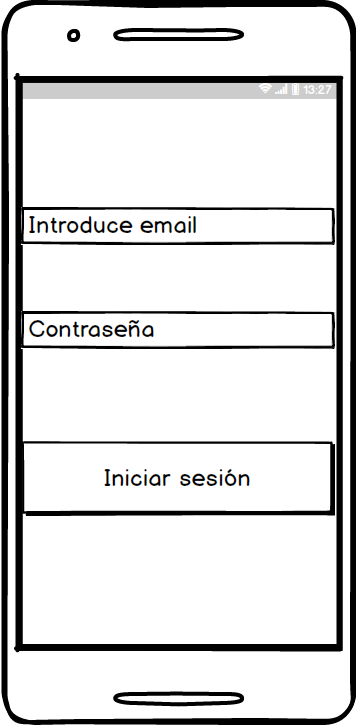
\includegraphics[width=6cm]{maqueta/Iniciar.png}
 \label{figura1}
\caption{Inisiar sesión}

\end{minipage}
\hspace{0.5cm} % Si queremos tener un poco de espacio entre las dos figuras
\begin{minipage}[b]{0.5\linewidth}
\centering
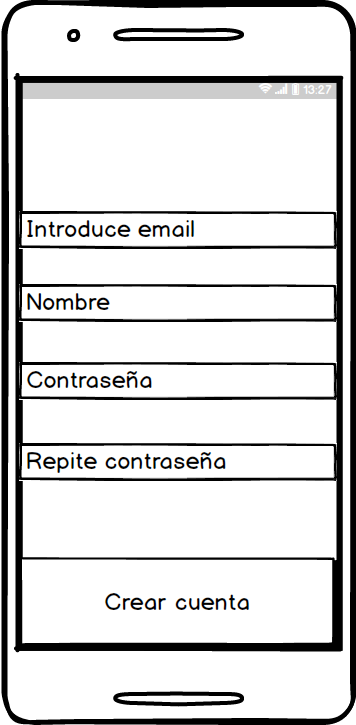
\includegraphics[width=6cm]{maqueta/Registrarse.png}
 \label{figura2}
\caption{Registrar usuario}

\end{minipage}
\end{figure}










	
	\begin{figure}[htbp]
\begin{minipage}[b]{0.5\linewidth} %Una minipágina que cubre la mitad de la página
\centering
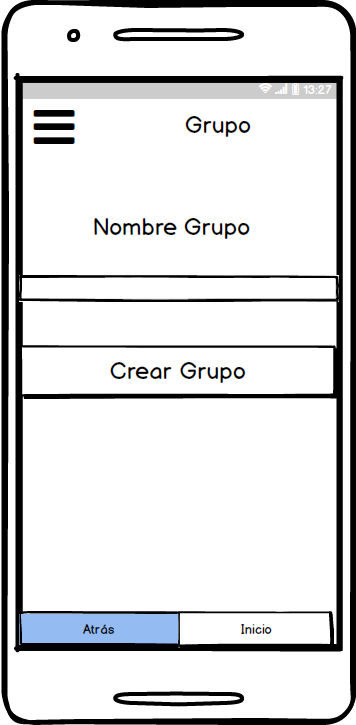
\includegraphics[width=6cm]{maqueta/Crear-Grupo.png}
 \label{figura1}
\caption{Crear grupo}

\end{minipage}
\hspace{0.5cm} % Si queremos tener un poco de espacio entre las dos figuras
\begin{minipage}[b]{0.5\linewidth}
\centering
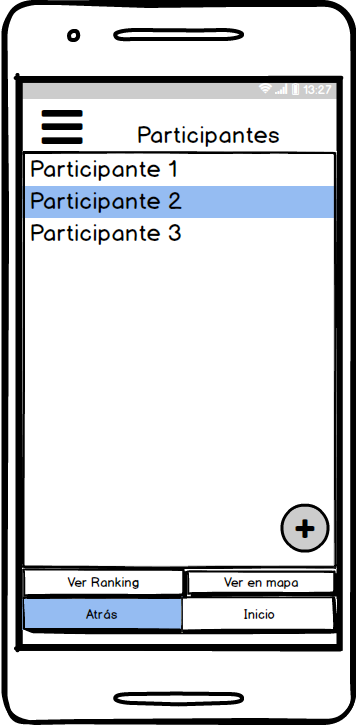
\includegraphics[width=6cm]{maqueta/Ver-Miembros-grupo.png}
 \label{figura2}
\caption{Añadir usuarios a grupo}

\end{minipage}
\end{figure}
	
	
	
	
	
	
	
	
	
	
	
	
	
	
	
	
	
	\begin{figure}[htbp]
\begin{minipage}[b]{0.5\linewidth} %Una minipágina que cubre la mitad de la página
\centering
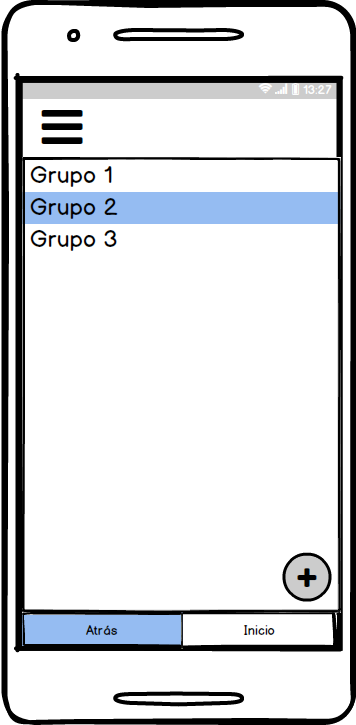
\includegraphics[width=6cm]{maqueta/lista-grupos.png}
 \label{figura1}
\caption{Listar grupos}

\end{minipage}
\hspace{0.5cm} % Si queremos tener un poco de espacio entre las dos figuras
\begin{minipage}[b]{0.5\linewidth}
\centering
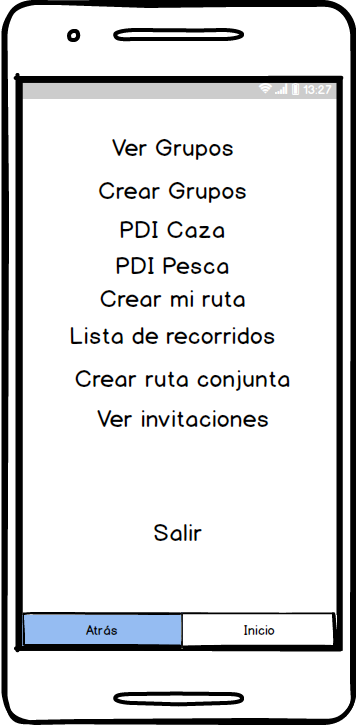
\includegraphics[width=6cm]{maqueta/opciones.png}
 \label{figura2}
\caption{Opciones generales}

\end{minipage}
\end{figure}
	















	\begin{figure}[htbp]
\begin{minipage}[b]{0.5\linewidth} %Una minipágina que cubre la mitad de la página
\centering
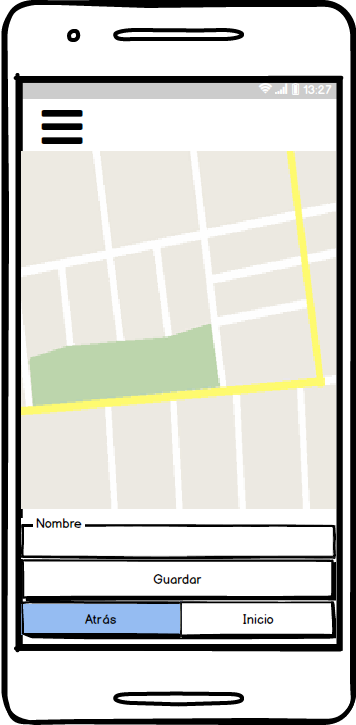
\includegraphics[width=6cm]{maqueta/pdi1.png}
 \label{figura1}
\caption{Crear PDI}

\end{minipage}
\hspace{0.5cm} % Si queremos tener un poco de espacio entre las dos figuras
\begin{minipage}[b]{0.5\linewidth}
\centering
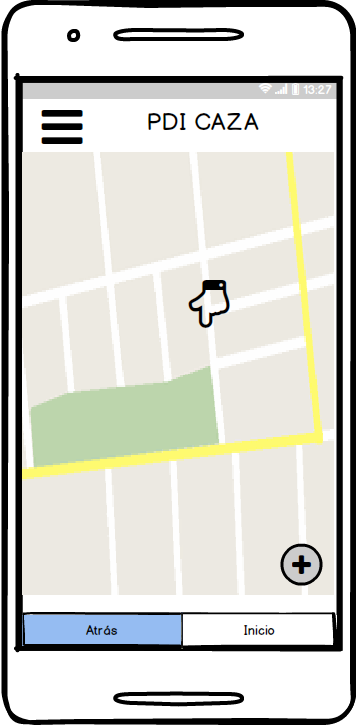
\includegraphics[width=6cm]{maqueta/pdi2.png}
 \label{figura2}
\caption{Visualizar PDIs}

\end{minipage}
\end{figure}
	

	\begin{figure}[htbp]
\begin{minipage}[b]{0.5\linewidth} %Una minipágina que cubre la mitad de la página
\centering
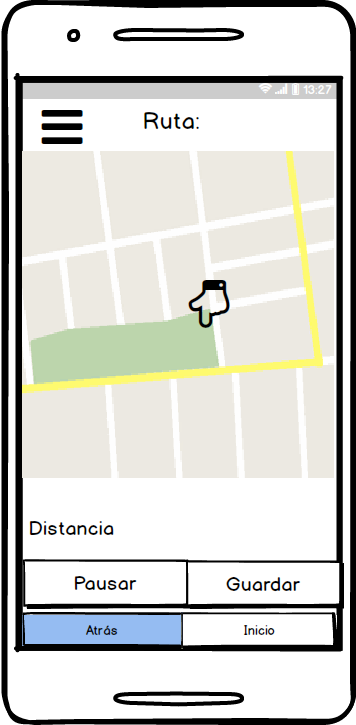
\includegraphics[width=6cm]{maqueta/Trayecto-actual.png}
 \label{figura1}
\caption{Ruta individual}

\end{minipage}
\hspace{0.5cm} % Si queremos tener un poco de espacio entre las dos figuras
\begin{minipage}[b]{0.5\linewidth}
\centering
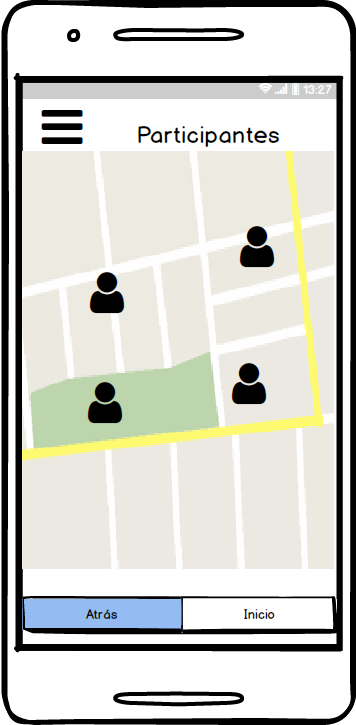
\includegraphics[width=6cm]{maqueta/Trayecto-actual-compartido.png}
 \label{figura2}
\caption{Ruta compartida}

\end{minipage}
\end{figure}


